\documentclass[t, 10pt]{beamer}
%%\documentclass[t,handout]{beamer}

\usepackage{graphicx}
\usepackage{epsfig}
\usepackage{psfrag}
\usepackage[english]{babel}
\usepackage{color}
%Mathematics packages
\usepackage{amsmath}
\usepackage{mathrsfs}
\usepackage{amsfonts}

\usepackage{enumerate}


\graphicspath{{./images/}} % Figures path - used in graphicx

\selectcolormodel{cmyk}

\mode<presentation>

%THEMES - Please refer to these chapters in the beamer documentation.
% Presentation themes : Chapter 15
% Color themes : Chapter 17
% Font themes : Chapter 18


\usetheme{Pittsburgh}
\usecolortheme{orchid}
\usefonttheme{default}

%---------------------------Title frame definition------------------------------------- 

\title{Managed Control of Composite Cloud Systems}
\author [Chris]{Christopher C. Lamb, Pramod A. Jamkhedkar, Gregory L. Heileman, and Chaouki T. Abdallah}
\institute[University of New Mexico]{
\inst {}Department of Electrical and Computer Engineering\\
University of New Mexico}
\date{June 10, 2011}
\titlegraphic{
\begin{figure} 

\includegraphics[width = 7cm]{UNM}
\end{figure}}

% Delete this, if you do not want the table of contents to pop up at
% the beginning of each subsection:
%\AtBeginSubsection[]
%{
%  \begin{frame}<beamer>
%    \frametitle{Outline}
%     \tableofcontents[currentsection,currentsubsection]
%  \end{frame}
%}

\begin{document}

\begin{frame}
\titlepage
\end{frame}

% This command will make the logo appear on all frames excluding the title frame.
\logo {
\includegraphics[width = 2.5cm]{UNM}}

\begin{frame}
\frametitle{Outline}
\tableofcontents 
\end{frame}

\section{UNM Informatics}
\begin{frame}
\frametitle{Areas of Study}

Our group:
\begin{itemize}
\item \textit{UNM Informatics}: Information security, theory, and architectures; this work is specific to information security 
\item \textit{Usage Management}: Control of how an artifact is used, covering everything \textit{after} access as well as controlling access itself
\end{itemize}
\pause

\textit{Motivation}: We believe people should have control over their own information.  Or past motivation for DRM work was to provide content control to content creators.  Doing so provides incentive for innovation, and improves quality of life for individuals and society as a whole over time.  We believe Usage Management provides the same benefits, and should be unobtrusive.
\newline
\newline
This motivation holds in this domain as well.
\pause

Acronyms:
\begin{itemize}
\item \textit{UM}: Usage Management
\item \textit{PMR}: Personal Medical Record (this is also electronic, in this case)
\end{itemize}

\end{frame}

\section{Usage Management and Cloud Systems}
\begin{frame}
\frametitle{Why is this important?}
Utility computing will certainly be the most pervasive future computing model \\
\pause
\begin{itemize}
\item \textit{Mainframes won!}
\pause
\begin{itemize}
\item Well, end devices are powerful
\item Cloud computing pervasive for \textit{convenience}, not \textit{technical necessity}.
\item \textit{Still resembles centralized models of the past}
\end{itemize}
\pause
\item \textit{People should control what they own}
\begin{itemize}
\item Access
\item Retention
\item Distribution
\end{itemize}
\pause \textit{Organizations should control what they pay for}
\begin{itemize}
\item Systems
\item Data
\item Records
\end{itemize}
\end{itemize}
\end{frame}

\begin{frame}
\frametitle{Problems}
So this is what we would like to see, but problems abound
\begin{itemize}
\item \textit{Scalability, performance, usability, infrastructural support...}
\end{itemize}
\pause

Started examining automation and ability to combine service level agreements (SLAs)
\begin{itemize}
\item \textit{Automation} \\
How we can automate control and enforcement
\item \textit{Combine} \\
How we can combine multiple SLAs into single SLAs
\end{itemize}
\pause

Surprisingly difficult...
\begin{itemize}
\item \textit{NP-Complete} \\
Simple generalized SLAs are equivalent to \textit{SAT}
\item \textit{Multiple Providers} \\
Difficult constant factors related to latency, etc.
\end{itemize}
 
\end{frame}

\section{Example Systems}
\begin{frame}
\frametitle{Single Provider, Feedback}

\begin{itemize}
\item \textit{Performance:} We will be adjusting a system within specific soft real-time frames.  Ergo, we need to be able to collect feedback measurements, process those measurements, and make decisions about how to respond to those measurements quickly in order to avoid falling out of compliance with any performance parameters to which we must adhere.
\item \textit{Accessibility:} In order to control component systems, we must be able to access those systems.  In order to do so within time constraints, we must be able to access those systems electronically as well; physical access requirements simply will not scale into this performance domain.
\item \textit{Controllability:} We must be able to access the appropriate control primitives on the systems we need to tune.  This will include accessing compute node generation and termination capabilities.  It would help if we could access node performance information and tune those nodes as well, though this is not required; we can emulate this by terminating nodes in one configuration and creating nodes with another to more adequately address performance needs.
\end{itemize}

\end{frame}

\begin{frame}
\frametitle{Single Provider, Feedback}

\begin{figure}
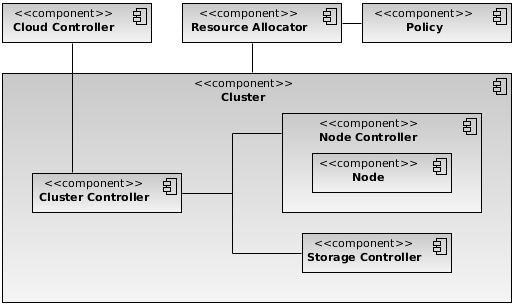
\includegraphics[width = 6cm]{Single-QoS}
\end{figure}

\end{frame}

\begin{frame}
\frametitle{Single Provider, Feedback}

\begin{itemize}
\item \textit{Cloud Controller} Provides an initial interface to administrative users to control the cloud.
\item \textit{Cluster Controller} Managed by the cloud controller, the cluster controller manages the resources of a single cluster. A given cloud may contain multiple clusters.
\item \textit{Storage Controller} Provides storage of system images and for other general storage needs.  This controller component is highly I/O sensitive.
\item \textit{Node Controller} Responsible for allocating, delivering, and managing individual compute nodes upon which client software runs.
\item \textit{Node} The compute node delivering services to end users and managed by the cluster's control infrastructure.  This is the primary computational resource accessed by users accessing managed cloud resources.
\item \textit{Policy} Quality of service terms the cloud provider has agreed to honor for the cloud customer with respect to system delivery, provisioning, and overall performance.
\item \textit{Resource Allocator} The component responsible for real-time tuning of the cloud system to maintain defined quality of service.
\end{itemize}

\end{frame}

\begin{frame}
\frametitle{Single Provider, Feedback with UM}

\begin{itemize}
\item \textit{Accessibility:} Data streamed through the cloud system must be able to be monitored and the accessibility of that stream needs to be dynamically tunable.  This implies that we need to be able to control routing and caching of all streaming data according to user specified conditions.  This also implies that we need to be able to control exactly which \textit{Node Controllers} are able to spawn which \textit{Nodes}.
\end{itemize}

\end{frame}

\begin{frame}
\frametitle{Single Provider, Feedback with UM}

\begin{figure}
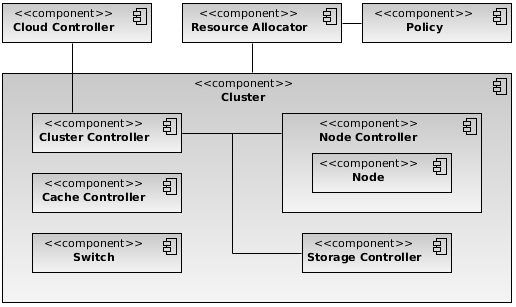
\includegraphics[width = 6.5cm]{Single-UM}
\end{figure}

\end{frame}

\begin{frame}
\frametitle{Single Provider, Feedback with UM}

\begin{itemize}
\item \textit{Cache Controllers:} Streaming network data, specifically media-centric streams, can and are cached by strategically located cache systems.  In order to control the read access of network data, we must be able to exercise explicit control over any caching systems in our infrastructure.
\item \textit{Switch:} Really any kind of hardware that controls the delivery of network data.  This component includes switches and routers primarily.  In order to control how data is accessed we must be able to control the locations to which it is delivered.
\end{itemize}

\end{frame}

\begin{frame}
\frametitle{Multiple Providers}

\begin{figure}
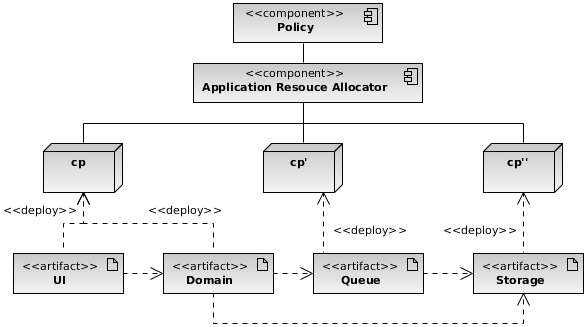
\includegraphics[width = 6cm]{Multiple}
\end{figure}

\end{frame}

\begin{frame}
\frametitle{Conclusions}

\end{frame}

%\bibliographystyle{plain}
%\bibliography{drm}

\end{document}

